\section{Results and Discussion} \label{sec:results_discussion}
\subsection{Results} \label{sec:results}
An alpha level of 0.05 was used for all statistical tests. Two-way analysis of variance (ANOVA) tests were used to test all hypotheses. Both \xQ{} and \xO had two levels (`present', `absent').

\paragraph{\ref{itm:H1}---Total Score}
       \begin{figure}[tb]
            \centering
            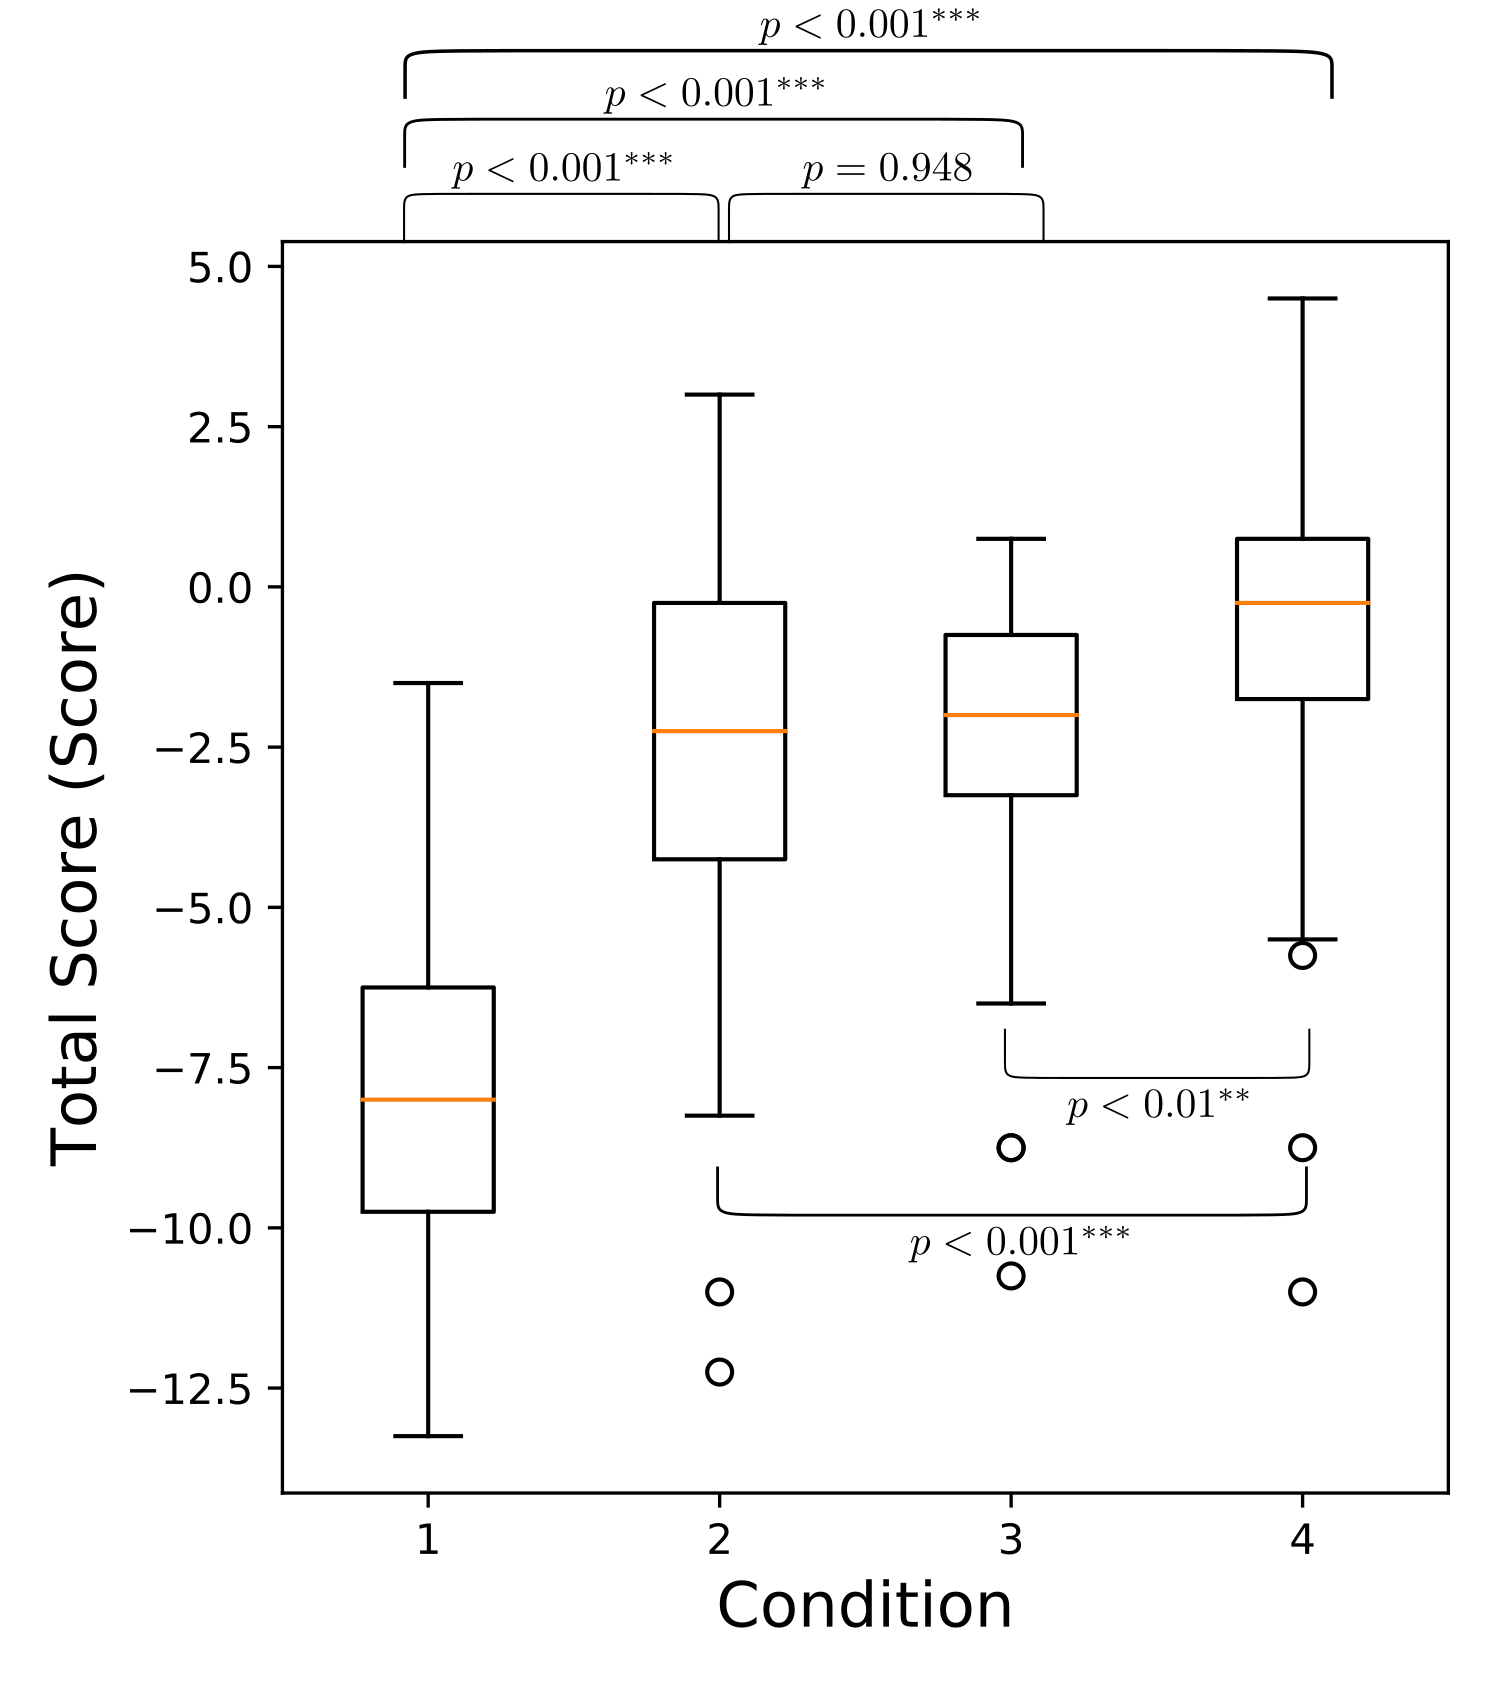
\includegraphics[width=0.7\linewidth]{Figures/total_score_box.png}
            \caption{Participants' cumulative total score by condition.}
            \label{fig:score_box}
       \end{figure}
A two-way analysis of variance was conducted on the influence of \xQ{} and \xO{} on the participant's total score. The main effect of \xQ{} was significant \Fratio{1}{251}{107.9}{0.001}. Participants in \xQ{} `present' conditions had significantly higher scores \MSD{-1.63}{3.06} than those in the \xQ{} `absent' conditions \MSD{-5.08}{3.61}. The main effect of \xO{} was also significant \Fratio{1}{251}{124.5}{0.001}. Participants in the \xO{} `present' conditions scored higher \MSD{-1.51}{2.63} than those in the \xO{} `absent' conditions \MSD{-5.23}{3.82}. The interaction effect was also significant \Fratio{1}{251}{26.4}{0.001}.

Post-hoc comparisons using Tukey's HSD test indicate that the \xQ{} `present', \xO{} `absent' condition \CMSD{\ref{itm:C2}}{-2.64}{3.10} results in a significantly higher score (\ps{0.001}) than in control \CMSD{\ref{itm:C1}}{-7.82}{2.50}. The score is also higher  in the \xO{} `present', \xQ{} `absent' condition \CMSD{\ref{itm:C3}}{-2.39}{2.26} with \ps{0.001}, and in the \xQ/\xO{} `present' condition \CMSD{\ref{itm:C4}}{-0.64}{2.70} with \ps{0.001}. The \xQ{} `present' condition (\ref{itm:C2}) is not significantly different from \xO{} `present' condition (\ref{itm:C3}) (\pns), but the scores of those in the \xQ/\xO{} `present' condition (\ref{itm:C4}) are significantly higher than either \xQ{} `present', or \xO{} `present' conditions (\ref{itm:C2}, \ref{itm:C2}) alone (\ps{0.001}, and \ps{0.01} respectively). See Fig.~\ref{fig:score_box} for visualization.

\paragraph{\ref{itm:H2}---Trust}
       \begin{figure}[tb]
            \centering
            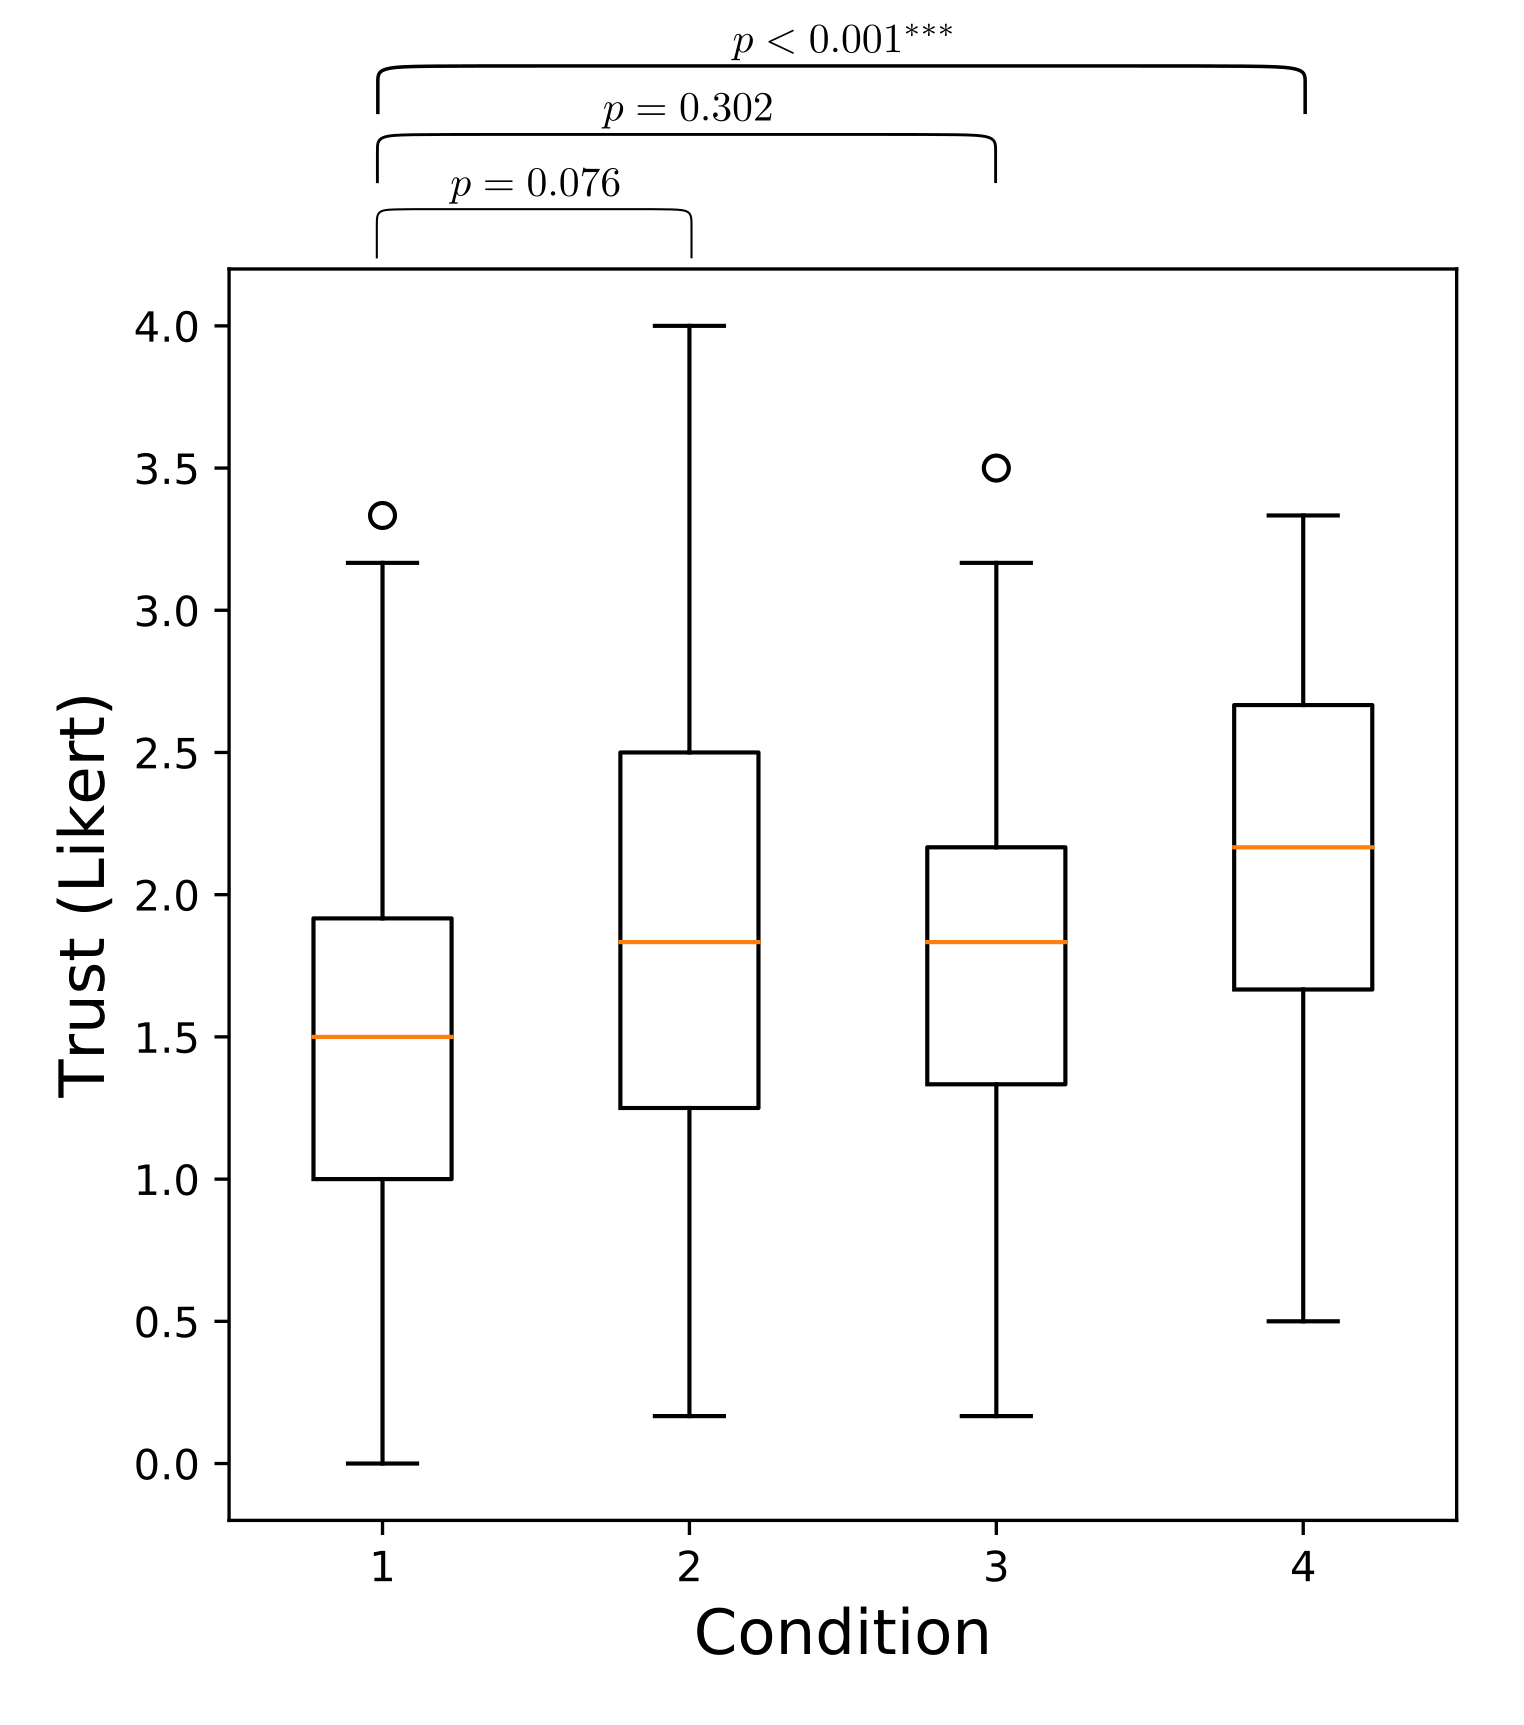
\includegraphics[width=0.7\linewidth]{Figures/trust_box.png}
            \caption{Participants' self-reported trust by condition.}
            \label{fig:trust_box}
       \end{figure}
Factor analysis of the survey questions indicated that survey questions 1,2,4,5,6, and 7 could be used in the same `Trust' scale with Cronbach's $\alpha = 0.87$ (see Appendix~\ref{sec:survey_questions} to see detailed question wording). Each participant's Likert responses from these questions were combined by taking their average; this data is shown in Fig.~\ref{fig:trust_box}.

Analysis of variance indicated that the main effects of \xQ{} were significant \Fratio{1}{251}{13.6}{0.001}. Participants in \xQ{} `present' conditions \MSD{2.04}{0.79} had significantly more trust than those in \xQ{} `absent' conditions \MSD{1.69}{0.75}. The main effects of \xO{} were also significant \Fratio{1}{251}{7.3}{0.01}. Those in \xO{} `present' conditions \MSD{1.99}{0.72} had higher trust than those in \xO{} absent conditions \MSD{1.73}{0.83}. The interaction effect was not significant \Frations{1}{251}{0.05}.

In Post-hoc analysis using Tukey's HSD the trust of participants in the \xQ{} `present', \xO{} `absent' condition \CMSD{\ref{itm:C2}}{1.89}{0.85} was found to be significantly higher than control \CMSD{\ref{itm:C1}}{1.57}{0.78} with $p<0.001$. The trust rating in the \xO{} `present', \xQ{} `absent' condition \CMSD{\ref{itm:C3}}{1.80}{0.70} was also higher than in control ($p<0.01$). The \xQ/\xO{} `present' condition \CMSD{\ref{itm:C4}}{2.17}{0.70} is significantly higher than control as well ($p<0.001$). Other interactions were not significant. See Fig.~\ref{fig:trust_box} for visualization.

\paragraph{\ref{itm:H3}---Average Task Time}
       % \begin{figure}[tb]
            % \centering
            % 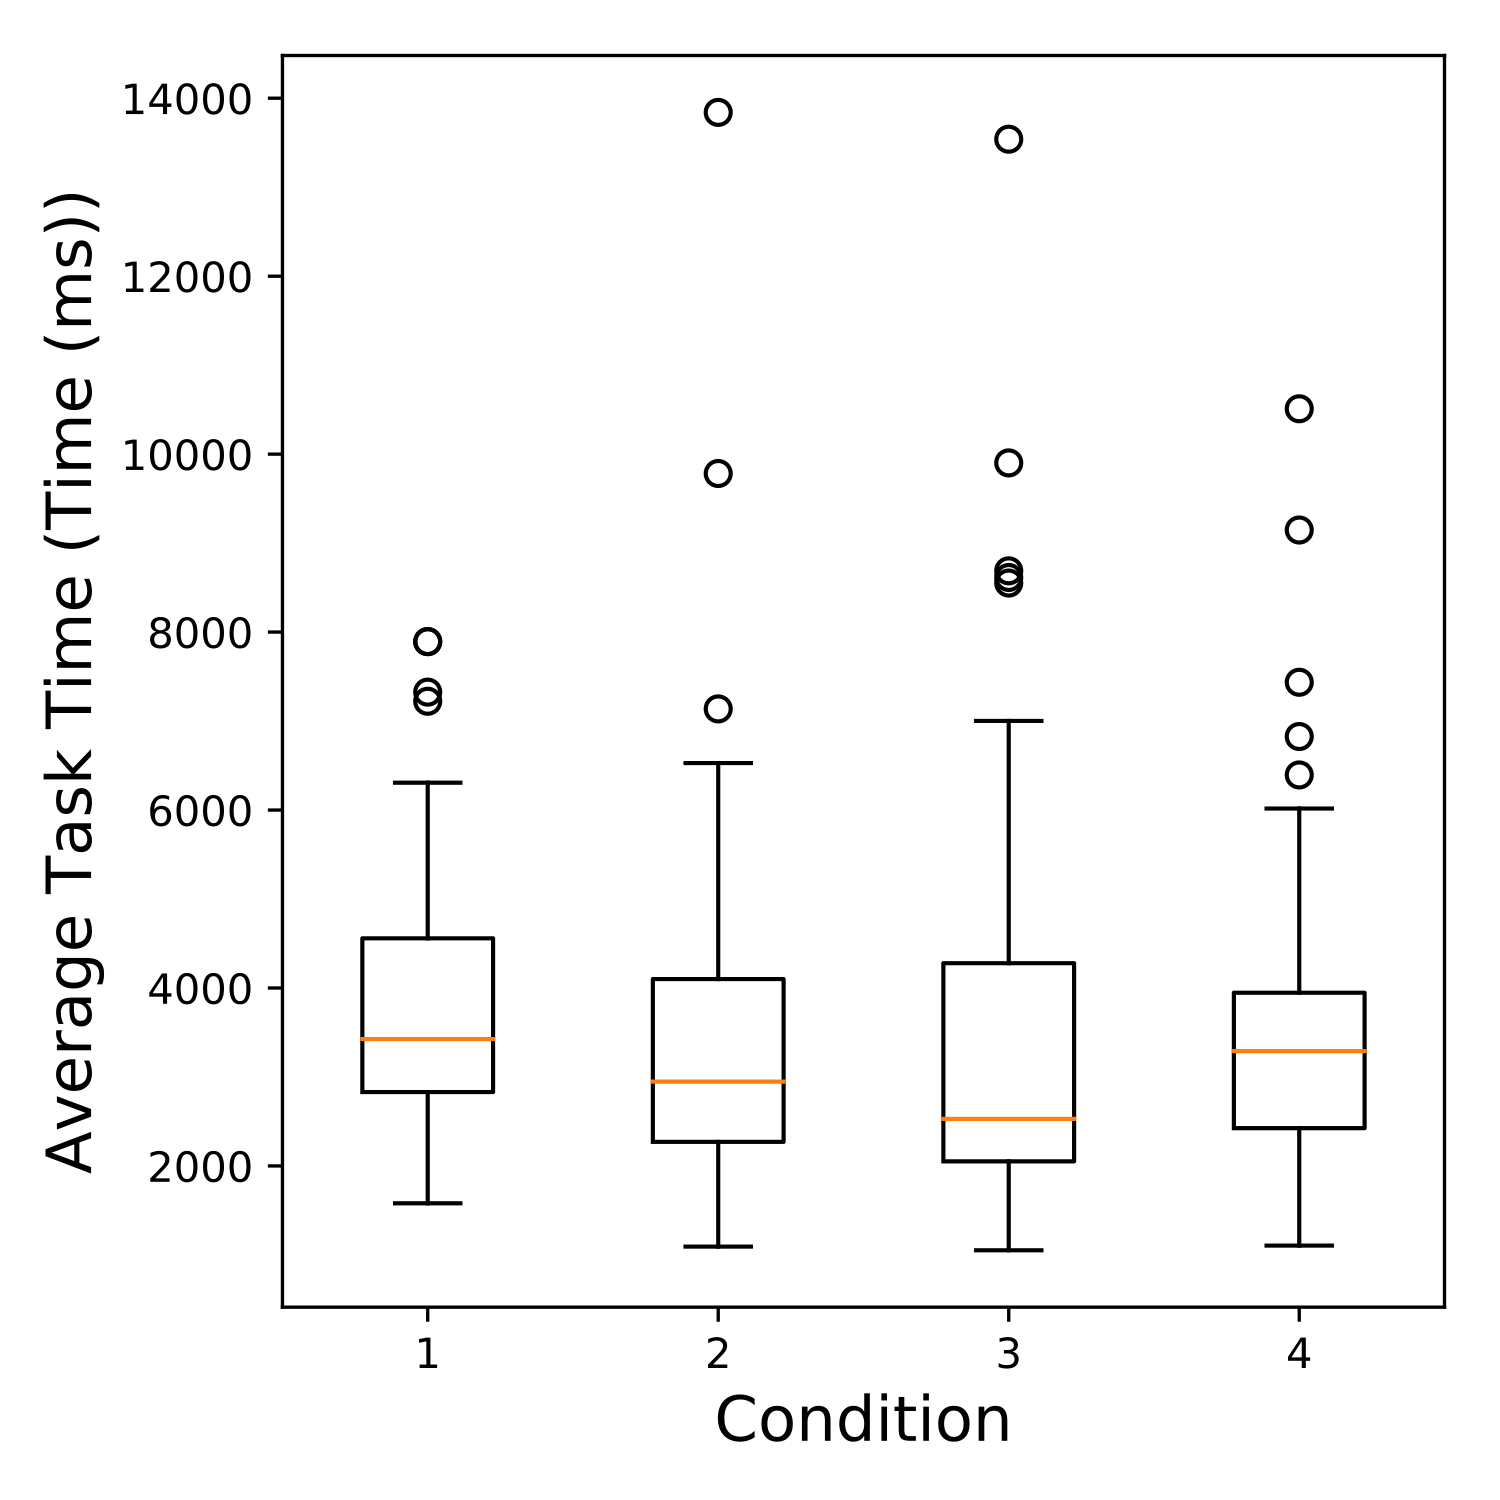
\includegraphics[width=0.8\linewidth]{Figures/avg_time_box.png}
            % \caption{\brett{WE COULD LEAVE THIS FIGURE OUT PROBABLY\ldots} Box plots showing the participants average task time by condition.}
            % \label{fig:time_box}
       % \end{figure}
Analysis of variance of the influence of \xQ{} and \xO{} on the participant's average task time was performed. The main effects of \xQ{} \Frations{1}{251}{0.64} and of \xO{} \Frations{1}{251}{0.06} were not found to be significant. The interaction effect was also not found to be significant \Frations{1}{251}{0.53}.

\subsection{Discussion} \label{sec:discussion}
The task was frustrating to several participants, one said: ``This feels rigged'', and another: ``I felt I had to decline the delivery too often''. Even so, the results show that the presence of \xQ{} and \xO{} helped the users to perform better on the task and get a higher total score. This was true individually in \ref{itm:C2}, and \ref{itm:C3} and even more so with both of the metrics `present' (\ref{itm:C4}). 

As reported above the differences in score between \ref{itm:C2}, and \ref{itm:C3} were not significantly different from each other. This reflects the balanced nature of the experiment data set (no single metric was more important than the other). Used in conjunction the UDT was able to convey the areas in which it had the most capability, and that resulted in condition \ref{itm:C4} having a significantly higher score than all other conditions (even though that involved declining more deliveries).

The effects of self-confidence metrics on user trust while significant, were not as strong as on the total score. Much of this can be attributed to the fact that this was a between-subjects study. Without a baseline experience it is impossible for participants to know how much they trust the UDT equipped with \xQ{} and/or \xO. We hypothesize that if the experiment would have been within-subjects the trust levels would have been much more different, this is left for future work. We also believe that this is the reason for the overall `low' trust ratings given by users in all conditions (the best condition \ref{itm:C4} has a mean average Likert response of 2.17 over the 6 questions included).

The survey responses more likely reflect some of the biases that participants had regarding how they thought the UDT \emph{should have done}. A few participants shared that they felt the delivery truck should have been able to `do better', this indicates that they still felt like they didn't have enough information to convince them that the UDT was actually trustworthy. This suggests that users need to understand more detail about the UDT's capabilities before they can be convinced to \emph{consciously} assign `trust' to the UDT. This is where other, more detailed, algorithmic assurances could come into play. For example an explanation system might communicate ``Solver Quality is low because the transition probability is very poor in this city''. Having said this, user performance was markedly different, and those who design autonomous systems must ask themselves which goals are more important: 1) more appropriate behaviors/actions, or 2) improving perceived trust; this experiment indicates that it is easier to influence user behavior than it is to influence their level of perceived trust, at least in isolation (i.e. a between-subjects situation such as this).

The fact that \xQ{} and \xO{} did not have a significant effect on the average time to complete tasks is somewhat surprising to us. The reasoning behind the hypothesis was that both \xQ{} and \xO{} are meant to offload some of the decision-making work from the user. However, in retrospect, \xQ{} and \xO{} are really presenting more nuanced information to the user that they \emph{would not have considered before}. For example, participants in the control condition likely had an implicit assumption that the UDT solver worked the same on every task (i.e. the latent \xQ{} was ``very good'' all of the time) since they had no real idea of any other possibility. On reflection, this experiment was not well suited to investigating changes in cognitive load. This also is left for future investigation.

These results are very promising in indicating that \famsec{} as an \emph{algorithmic assurance} elicits \emph{appropriate behavior}. User behaviors (indicated by decisions, and ultimately the score in this work) are really the objective measures of the effects of the assurances. It is also promising that self-reported `trust' levels in condition \ref{itm:C4} were significantly higher as well; however in order to truly understand the effects on trust we believe it would be more `fair' to perform a within-subjects study to measure changes in trust between conditions to have a more accurate baseline of trust for the control condition.

One might argue that the `Donut Delivery' task is too simple to be interesting. There are a few different reasons that it was selected: 1) Using a more complex problem would introduce too many confounding factors that could limit the possibility of accurately observing effects of the \famsec{} metrics; 2) Having a simple task is desirable when trying to run an experiment a large, diverse, group of non-experts; 3) If support for the hypotheses were found in this experiment then more realistic, complex, and expensive experiments could be run in the future.

% \brett{some interesting comments to possibly bring up}
% Interesting comments: 1) \emph{``I felt like I had to decline the delivery too often''} 2) \emph{``I tried to figure it out from the map sometimes, but the truck was right more often than me''}, 3) \emph{``I thought that the proximity to the motorcycle gang would be a factor but it was very hard to predict''}, 4) \emph{``This feels rigged >.>''}, 5) \emph{``I enjoyed completing the HIT however the delivery truck should have been able to make more deliveries considering the short nature of the imagined route''} 5) \emph{``I think the system works well whenever it is trusted. I made the mistake of relying too much on the visible map. Things were better when using entire system.''}
%
% As one participant noted: ``I think the system works well whenever it is trusted. I made the mistake of relying too much on the visible map. Things were better when using entire system.''
